\listfiles
\documentclass[3p]{elsarticle}

\usepackage{lineno,hyperref}
\modulolinenumbers[5]

\journal{Applied Machine Learning Course}

%%%%%%%%%%%%%%%%%%%%%%%
%% Bibliography styles
%%%%%%%%%%%%%%%%%%%%%%%
%% To change the style, put a % in front of the second line of the current style and
%% remove the % from the second line of the style you would like to use.
%%%%%%%%%%%%%%%%%%%%%%%

% Numbered
% \bibliographystyle{model1-num-names}

%% Numbered without titles
% \bibliographystyle{model1a-num-names}

%% Harvard
% \bibliographystyle{model2-names}\biboptions{authoryear}

%% Vancouver numbered
% \usepackage{numcompress}\bibliographystyle{model3-num-names}

%% Vancouver name/year
% \usepackage{numcompress}\bibliographystyle{model4-names}\biboptions{authoryear}

%% APA style
% \bibliographystyle{model5-names}\biboptions{authoryear}

%% AMA style
% \usepackage{numcompress}\bibliographystyle{model6-num-names}

%% `Elsevier LaTeX' style, distributed in TeX Live 2019
\bibliographystyle{elsarticle-num}
% \usepackage{numcompress}\bibliographystyle{elsarticle-num-names}
% \bibliographystyle{elsarticle-harv}\biboptions{authoryear}
%%%%%%%%%%%%%%%%%%%%%%%

%%%%%%%%%%%%%%%%%%%%%%%%%%%%%%%%%%%%%%%%%%%%%%%%%%%%%%%%%%%%%%%
% DO NOT EDIT ANYTHING ABOVE THIS LINE
% EXCEPT IF YOU LIKE TO USE ADDITIONAL PACKAGES
%%%%%%%%%%%%%%%%%%%%%%%%%%%%%%%%%%%%%%%%%%%%%%%%%%%%%%%%%%%%%%%


\usepackage{comment}

\newcommand\blfootnote[1]{%
  \begingroup
  \renewcommand\thefootnote{}\footnote{#1}%
  \addtocounter{footnote}{-1}%
  \endgroup
}

\begin{document}

\begin{frontmatter}

%%%%%%%%% TITLE
%\title{Applied Machine Learning: Disease Symptom Prediction\\}
\title{Applied Machine Learning \\ \huge{\textbf{Disease Symptom Prediction}}}

%%%%%%%%% AUTHORS
\author{Louis Simon Spatscheck, Aikaterini Vasilopoulou, \\ 
Léandre Pablo Delphin Göblyös, Dominik Pastuszka Malek}
\let\thefootnote\relax\footnotetext{\textit{Email adresses:} author1@student.sdu.dk, author2@student.sdu.dk, author3@student.sdu.dk, dpast24@student.sdu.dk}

\begin{comment}
\author{Louis Simon Spatscheck}
\ead{author1@student.sdu.dk}
\author{Aikaterini Vasilopoulou}
\ead{author2@student.sdu.dk}
\author{Léandre Pablo Delphin Göblyös}
\ead{author3@student.sdu.dk}
\author{Dominik Pastuszka Malek}
\ead{dpast24@student.sdu.dk}
\end{comment}

%%%%%%%%% ABSTRACT
\begin{abstract}
The abstract for your project goes here. The length of the abstract should be about 200 words. Tips for writing a good abstract can be found at  \url{https://www.ncbi.nlm.nih.gov/pmc/articles/PMC3136027/}. \\

%\noindent Link to dataset: 
%\begin{center}
%    \href{https://www.kaggle.com/datasets/itachi9604/disease-symptom-description-dataset}{Disease Symptom Prevention (Kaggle)}
%\end{center}

\noindent Link to \textit{GitHub} repository containing the dataset and all code developed for this project:
\begin{center}
    \href{https://github.com/domipm/AML-Disease-Symptom}{Applied Machine Learning - Disease Symptom Prevention (GitHub)}
\end{center}

\end{abstract}


\end{frontmatter}




% MAIN ARTICLE GOES BELOW
%%%%%%%%%%%%%%%%%%%%%%%%%%%%%%%%%%%%%%%%%%%%%%%%%%%%%%%%%%%%%%%




%%%%%%%%% BODY TEXT
\section{Introduction}

\begin{itemize}
    \item Introduce Machine Learning and its applications in healthcare.
    \item Introduce the dataset and its relevance to the project + explain dataset with visuals
    \item Introduce the main goal of the project.
    \item Introduce the structure of the report.
\end{itemize}

\cite{peimankar2017evolutionary}

\section{Related Work}

\begin{itemize}
    \item Don't know if we need that section, any ideas ?
\end{itemize}

\begin{figure}[t]
\begin{center}
   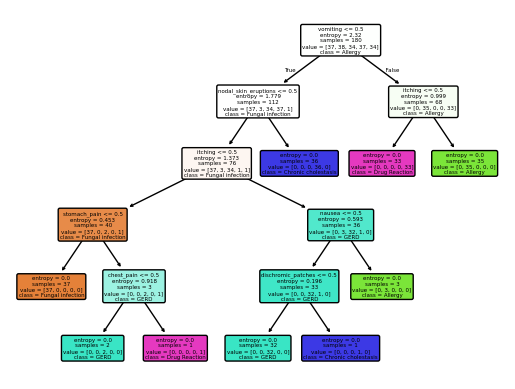
\includegraphics[width=0.8\linewidth]{images/output.png}
\end{center}
   \caption{Example illustrating how to get BibTeX references from
   Google Scholar.}\label{fig:google-scholar}
\end{figure}


\begin{table}[h]
\begin{center}
\begin{tabular}{lc}

Method & Accuracy \\
\hline\hline
Method 1 & $70 \pm 3$ \% \\
Method 2 & $76 \pm 3$ \% \\

\end{tabular}
\end{center}\label{tab:some-table}
\caption{This is an example of a table.}
\end{table}

\section{Proposed Method}

\begin{itemize}
    \item Describe the transformations to the dataset you are using. One-Hot Encoding. Also trying other transformations (balancing) ?
    \item Describe the methods you are using (DT, RF, SVM, LR, NN). You can use a table to summarize the methods.
    \item Describe the evaluation metrics you are using (acc, confusion, ROC). You can use a table to summarize the metrics.
\end{itemize} 


\section{Experiments}

\begin{itemize}
    \item Describe Binary Classification experiments. Modelsetups and hyperparameter tuning (gridSearch)
    \item Describe Multi-class Classification on subset, which parameters are optimized. show parameter tuning? (gridSearch)
    \item Describe Multi-class Classification on full dataset, which parameters are optimized. show parameter tuning? (gridSearch)
    \item More Experiments?
\end{itemize}
\subsection{Binary Classification}


\subsection{Multi-class Classification}


\section{Results and Discussion}

\begin{itemize}
    \item Describe the results of the experiments. You can use tables and figures to summarize the results.
    \item Discuss the results. What do they mean? How do they compare to other methods? What are the limitations?
\end{itemize}

\section{Conclusions}

\begin{itemize}
    \item Summarize the main findings of the project.
    \item Discuss the implications of the findings. Is this suitable for real-world applications?
    \item Discuss the limitations of the project and future work.
\end{itemize}

\section{Acknowledgements}


\section{Contributions}

Describe the contributions of each team member who worked on this project.




\bibliography{mybibfile}

\end{document}